\documentclass[11pt]{article}
\usepackage{alltt, amssymb, amsfonts, amsmath, color, fancyhdr, graphicx, mathrsfs, setspace, tikz, titling, ulem}

% decrease margins
\addtolength{\oddsidemargin}{-.875in}
\addtolength{\evensidemargin}{-.875in}
\addtolength{\textwidth}{1.75in}
\addtolength{\topmargin}{-.875in}
\addtolength{\textheight}{1.75in}

\def\A{\mathcal A}\def\B{\mathcal B}\def\C{\mathcal C}\def\D{\mathcal D}\def\E{\mathcal E}\def\F{\mathcal F}\def\G{\mathcal G}\def\I{\mathcal I}\def\J{\mathcal J}\def\L{\mathcal L}\def\M{\mathcal M}\def\N{\mathcal N}\def\O{\mathcal O}\def\P{\mathcal P}\def\Q{\mathcal Q}\def\R{\mathcal R}\def\S{\mathcal S}\def\T{\mathcal T}\def\W{\mathcal W}\def\V{\mathcal V}\def\X{\mathcal X}\def\Y{\mathcal Y}\def\Z{\mathcal Z}
\def\mN{\mathbb N}\def\mR{\mathbb R}\def\mS{\mathbb S}
\def\bE{{\bf E}}
\def\bx{{\bf x}}
\def\prob{\mbox{\bf prob}}\def\tr{\mbox{\bf tr}}
\def\l{\left}\def\r{\right}\def\lf{\lfloor}\def\rf{\rfloor}
\def\un{\underline}
\def\theat{\theta}\def\lambad{\lambda}\def\lamda{\lambda}
\def\minimize{\mbox{minimize}\hspace{4mm}}\def\maximize{\mbox{maximize}\hspace{4mm}}\def\subjectto{\mbox{subject to}\hspace{4mm}}

\begin{document}
\thispagestyle{empty}
\begin{center}
\un{IMSA Data Mining Intersession}\\
\bf{Day 2 Worksheet}\\
\it{$k$-Nearest Neighbors}\\
\end{center}
We simulated a toy data set of 20 points, plotted below. Each data point has an observation in two variables: $x$ and $y$. The red data points (1 -- 10) where generated differently than the blue data points (11 -- 20). Your task in this exercise is to implement $k$-Nearest Neighbors by hand to classify new data points 21 -- 23 (unlabeled, colored black) as either red or blue.
\begin{center}
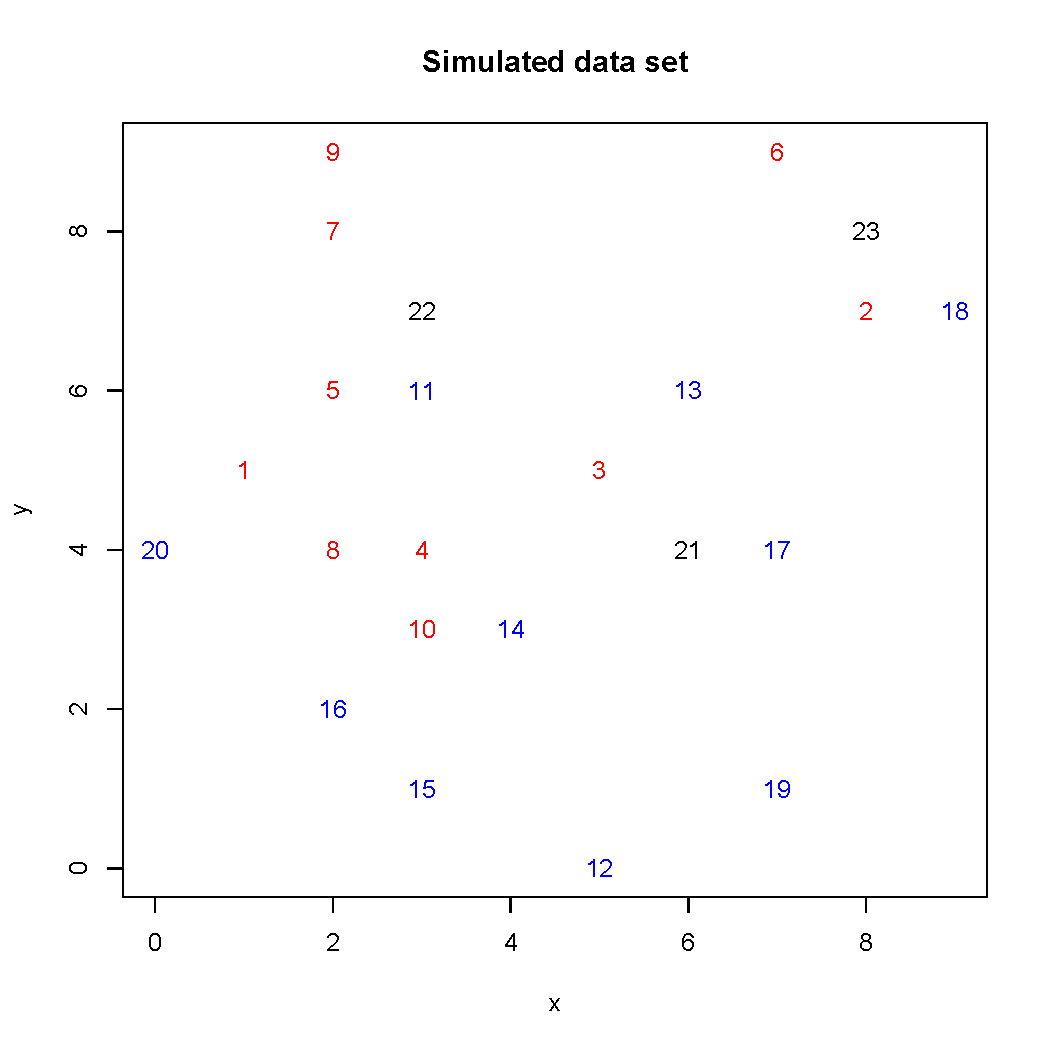
\includegraphics[scale = 0.6]{plot.pdf}
\hspace{1cm}
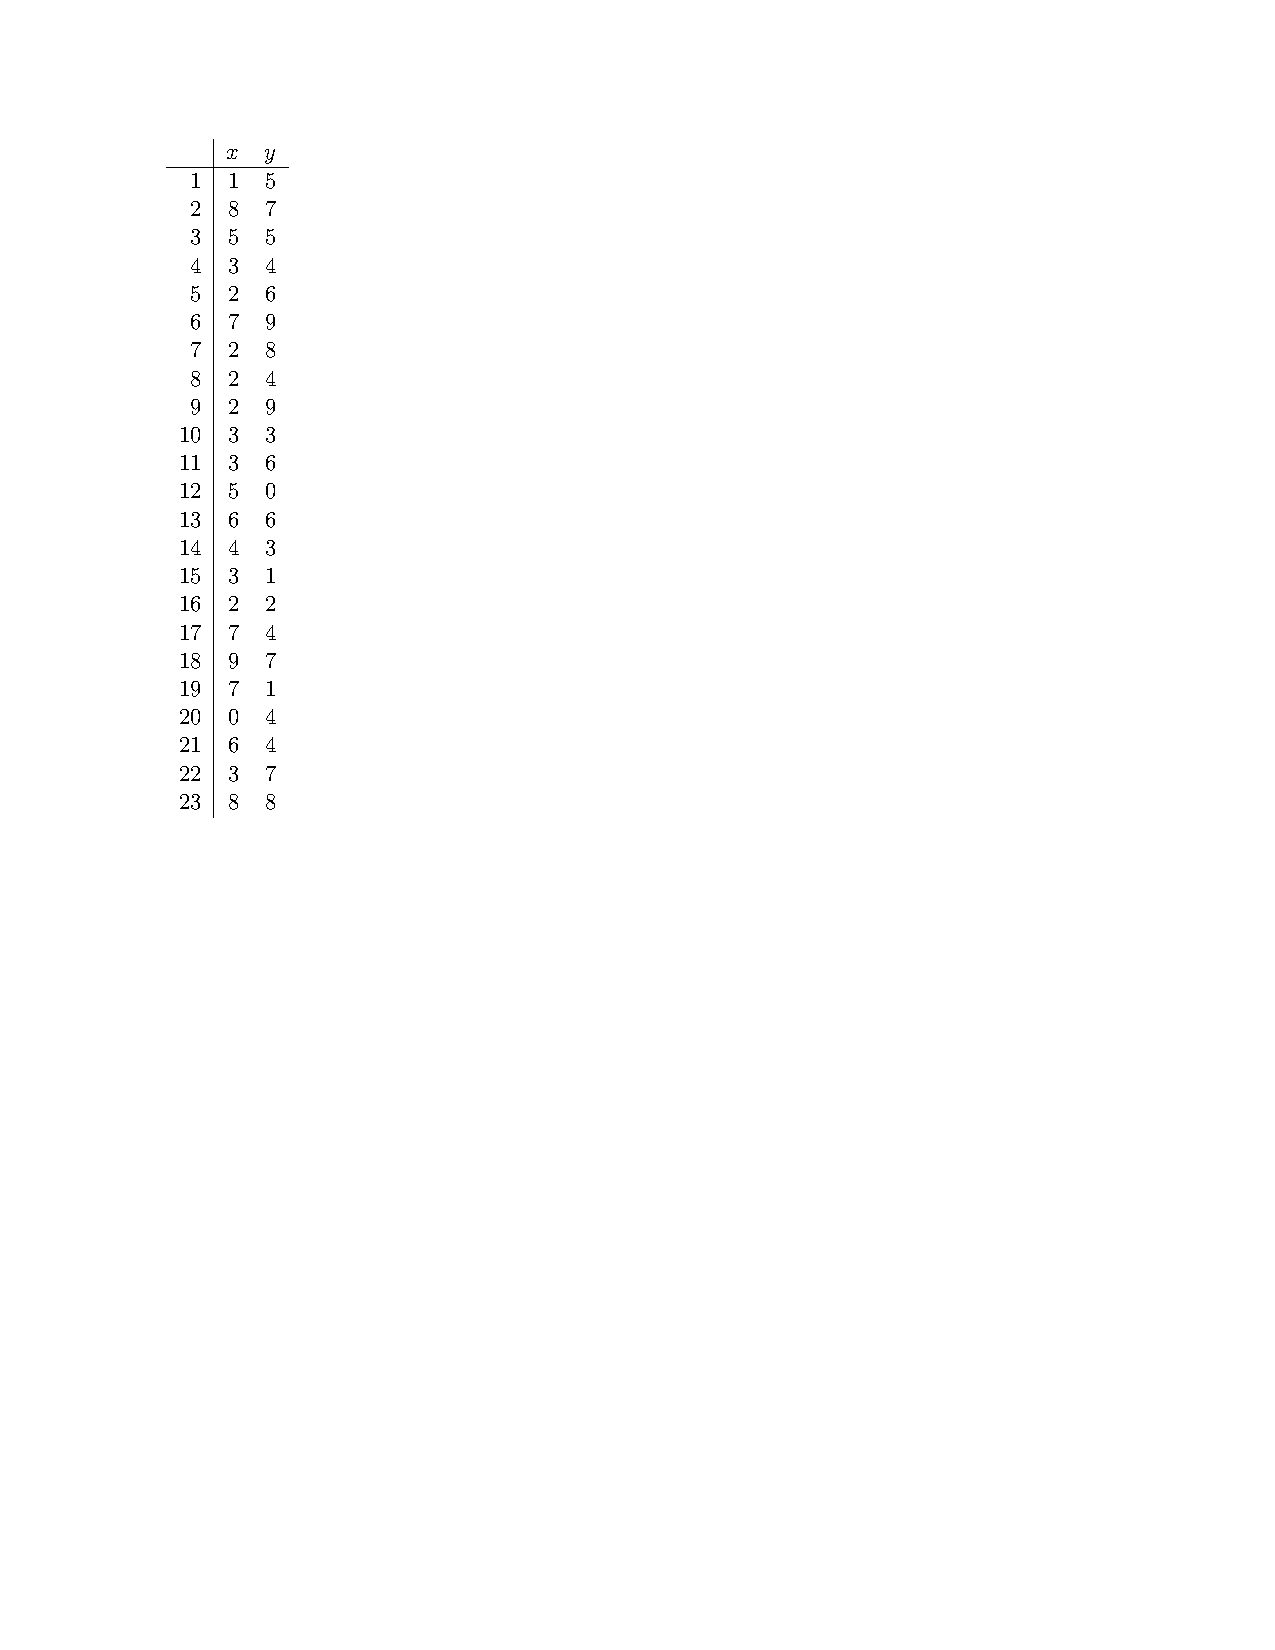
\includegraphics[scale = 0.9]{table.pdf}
\end{center}
The closer two points are to each other, the more similar they are. Use squared Euclidean distance: The distance between two points $(x_1, y_1)$ and $(x_2, y_2)$ is $(x_1 - x_2)^2 + (y_1 - y_2)^2$.
\begin{enumerate}
\item Classify the new data point 21 using 1-, 3-, 7- and 19-Nearest Neighbors.\\~\\
\item Classify the new data point 22 using 1-, 3-, 7- and 19-Nearest Neighbors.\\~\\
\item Classify the new data point 23 using 1-, 3-, 7- and 19-Nearest Neighbors.\\~\\
\item Why did we only consider odd values of $k$ in the above exercises?\\~\\
\item What is a benefit of using a large value for $k$? What is a benefit of using a small value for $k$?
\end{enumerate}
\end{document}